\documentclass[12pt,a4paper]{article}

% ─── Packages ────────────────────────────────────────────────────────────────
\usepackage[utf8]{inputenc}
\usepackage[T1]{fontenc}
\usepackage{geometry}
\usepackage{graphicx}
\usepackage{float}
\usepackage{listings}
\usepackage{xcolor}
\usepackage{booktabs}
\usepackage{hyperref}
\usepackage{caption}
\usepackage{parskip}
\usepackage{titlesec}
\usepackage{fancyhdr}
\usepackage{array}

% ─── Page Layout ─────────────────────────────────────────────────────────────
\geometry{margin=1in}
\setlength{\parindent}{0pt}
\setlength{\parskip}{6pt}

% ─── Header / Footer ─────────────────────────────────────────────────────────
\pagestyle{fancy}
\fancyhf{}
\rhead{Lab 3: Kubernetes Orchestration}
\lhead{Nabin Ranabhat (078BCT050)}
\cfoot{\thepage}

% ─── Code Listing Style ───────────────────────────────────────────────────────
\definecolor{codebg}{RGB}{245,245,245}
\definecolor{codeframe}{RGB}{200,200,200}
\definecolor{keyword}{RGB}{0,0,180}
\definecolor{comment}{RGB}{0,128,0}
\definecolor{string}{RGB}{163,21,21}

\lstdefinestyle{dockerstyle}{
  backgroundcolor=\color{codebg},
  frame=single,
  rulecolor=\color{codeframe},
  basicstyle=\ttfamily\small,
  keywordstyle=\color{keyword}\bfseries,
  commentstyle=\color{comment},
  stringstyle=\color{string},
  breaklines=true,
  breakatwhitespace=true,
  tabsize=2,
  showstringspaces=false,
  captionpos=b,
}

\lstdefinestyle{yamlstyle}{
  backgroundcolor=\color{codebg},
  frame=single,
  rulecolor=\color{codeframe},
  basicstyle=\ttfamily\small,
  keywordstyle=\color{keyword}\bfseries,
  commentstyle=\color{comment},
  stringstyle=\color{string},
  breaklines=true,
  tabsize=2,
  showstringspaces=false,
  captionpos=b,
}

\lstdefinestyle{bashstyle}{
  backgroundcolor=\color{codebg},
  frame=single,
  rulecolor=\color{codeframe},
  basicstyle=\ttfamily\small,
  breaklines=true,
  tabsize=2,
  showstringspaces=false,
  captionpos=b,
}

% ─── Hyperlink Style ─────────────────────────────────────────────────────────
\hypersetup{
  colorlinks=true,
  linkcolor=blue,
  urlcolor=blue,
  citecolor=blue,
}

% ─── Section Title Formatting ────────────────────────────────────────────────
\titleformat{\section}{\large\bfseries}{\thesection}{1em}{}
\titleformat{\subsection}{\normalsize\bfseries}{\thesubsection}{1em}{}

% ─── Helper: screenshot placeholder ─────────────────────────────────────────
% Usage: \screenshot{images/filename.png}{Caption text}{label}
\newcommand{\screenshot}[3]{%
  \begin{figure}[H]
    \centering
    \fbox{%
      \begin{minipage}{0.85\textwidth}
        \centering
        \vspace{0.4cm}
        \textit{\small [Screenshot placeholder: \texttt{#1}]}\\[4pt]
        \textit{\small Add screenshot and replace with: \texttt{\textbackslash includegraphics[width=0.85\textwidth]\{#1\}}}
        \vspace{0.4cm}
      \end{minipage}%
    }
    % ---- Once you have the screenshot, replace the \fbox block above with: ----
    % \includegraphics[width=0.85\textwidth]{#1}
    \caption{#2}
    \label{fig:#3}
  \end{figure}
}

% =============================================================================
\begin{document}
% =============================================================================

% ─── Title Page ──────────────────────────────────────────────────────────────
\begin{titlepage}
  \centering
  \vspace*{2cm}
  {\LARGE\bfseries Lab 3: Kubernetes Container Orchestration Lab Report\par}
  \vspace{1.5cm}
  {\large Nabin Ranabhat (078BCT050)\par}
  \vspace{0.5cm}
  {\large Department of Electronics and Computer Engineering\par}
  \vspace{0.5cm}
    {\large Pulchowk Engineering Campus\par}
    {\large IOE, Tribhuvan University\par}
  \vfill
\end{titlepage}

% ─── Table of Contents ───────────────────────────────────────────────────────
\tableofcontents
\newpage

% =============================================================================
\section{Introduction}
% =============================================================================

Kubernetes (K8s) is an open-source container orchestration platform that automates
the deployment, scaling, and management of containerised applications. Building upon
the foundational containerisation skills acquired in Lab~2, this lab extends the
workflow by deploying the same multi-service application---frontend (Nginx),
backend (Flask/Python), and database (MySQL)---onto a local Kubernetes cluster
managed by \textbf{Minikube}.

Unlike Docker Compose, which targets single-host environments, Kubernetes introduces
abstractions such as \textit{Pods}, \textit{Deployments}, \textit{Services}, and
\textit{ConfigMaps} that are designed for production-grade, multi-node deployments.
This practical exercise covers the complete Kubernetes workflow from cluster
initialisation to service exposure.

% =============================================================================
\section{Objectives}
% =============================================================================

\begin{itemize}
  \item Install and configure Minikube for local Kubernetes development.
  \item Build custom Docker images and load them into Minikube.
  \item Author Kubernetes manifest files (YAML) for Deployments and Services.
  \item Deploy the multi-container application stack on Kubernetes.
  \item Configure inter-service communication using Kubernetes DNS.
  \item Verify application health using \texttt{kubectl} commands.
  \item Explore Kubernetes networking concepts including NodePort and ClusterIP.
\end{itemize}

% =============================================================================
\section{Tools and Technologies Used}
% =============================================================================

\begin{itemize}
  \item Ubuntu Linux (Host Operating System)
  \item Docker Engine (Image Build Tool)
  \item Minikube v1.32+ (Local Kubernetes Cluster)
  \item kubectl (Kubernetes CLI)
    \item Python 3.11 / Slim (Backend Runtime)
  \item Nginx Alpine (Frontend Web Server)
  \item MySQL 8 (Relational Database)
    \item Kubernetes ConfigMap and Secret objects
\end{itemize}

% =============================================================================
\section{Background: Key Kubernetes Concepts}
% =============================================================================

\begin{center}
\begin{tabular}{>{\bfseries}p{3cm} p{10cm}}
\toprule
Concept & Description \\
\midrule
Pod        & Smallest deployable unit; wraps one or more containers. \\
 Deployment & Manages a desired number of Pod replicas with rolling-update support. \\
Service    & Stable network endpoint that load-balances traffic to Pods. \\
ClusterIP  & Default Service type; only reachable within the cluster. \\
NodePort   & Exposes a Service on a static port of each cluster node. \\
ConfigMap  & Stores non-sensitive configuration as key-value pairs. \\
 Secret     & Stores sensitive data (passwords, tokens) in base64 encoding. \\
Namespace  & Logical partition for isolating resources within a cluster. \\
\bottomrule
\end{tabular}
\end{center}

% =============================================================================
\section{Implementation Details}
% =============================================================================

% ─────────────────────────────────────────────────────────────────────────────
\subsection{Minikube Installation and Cluster Initialisation}
% ─────────────────────────────────────────────────────────────────────────────

Minikube was installed using the official binary release, and the cluster was
started with the Docker driver. The application images were then built locally
and loaded into the Minikube runtime:

\begin{lstlisting}[style=bashstyle, caption={Minikube installation and cluster start}]
# Install Minikube
curl -LO https://storage.googleapis.com/minikube/releases/latest/minikube-linux-amd64
sudo install minikube-linux-amd64 /usr/local/bin/minikube

# Install kubectl
sudo snap install kubectl --classic

# Start the local cluster
minikube start --driver=docker

# Build backend image
docker build -t lab2-backend:latest ./backend

# Build frontend image
docker build -t lab2-frontend:latest ./frontend

# Load images into Minikube
minikube image load lab2-backend:latest
minikube image load lab2-frontend:latest

# Verify images are available locally
docker images | grep lab2
\end{lstlisting}

\begin{figure}[H]
  \centering
  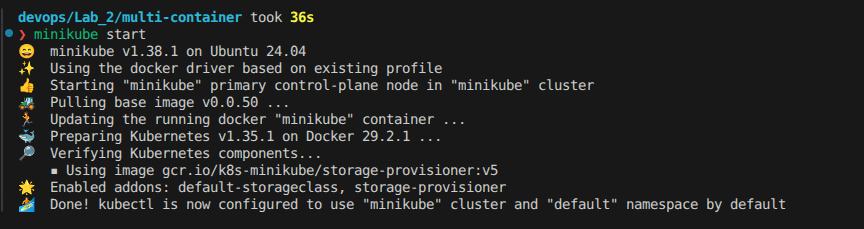
\includegraphics[width=0.85\textwidth]{images/minikube_start.png}
  \caption{Minikube cluster successfully started and node in \texttt{Ready} state}
  \label{fig:minikube_start}
\end{figure}
% What to capture: terminal output of `minikube start` showing "Done! kubectl
% is now configured to use minikube" and `kubectl get nodes` showing STATUS=Ready.

\begin{figure}[H]
  \centering
  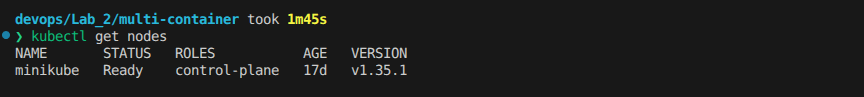
\includegraphics[width=0.85\textwidth]{images/kubectl_get_nodes.png}
  \caption{Kubernetes node status after cluster startup}
  \label{fig:kubectl_get_nodes}
\end{figure}

% ─────────────────────────────────────────────────────────────────────────────
\subsection{Building and Pushing Docker Images}
% ─────────────────────────────────────────────────────────────────────────────

The custom images from Lab~2 were rebuilt locally and loaded into Minikube so
that the Kubernetes cluster can use them without a remote container registry.

\begin{lstlisting}[style=bashstyle, caption={Build images inside Minikube's Docker context}]
# Point shell to Minikube's Docker daemon
eval $(minikube docker-env)

# Build backend image
docker build -t lab2-backend:latest ./backend

# Build frontend image
docker build -t lab2-frontend:latest ./frontend

# Load images into Minikube
minikube image load lab2-backend:latest
minikube image load lab2-frontend:latest

# Verify images are available locally
docker images | grep lab2
\end{lstlisting}

% ── SCREENSHOT: Docker build in Minikube ────────────────────────────────────
\begin{figure}[H]
  \centering
  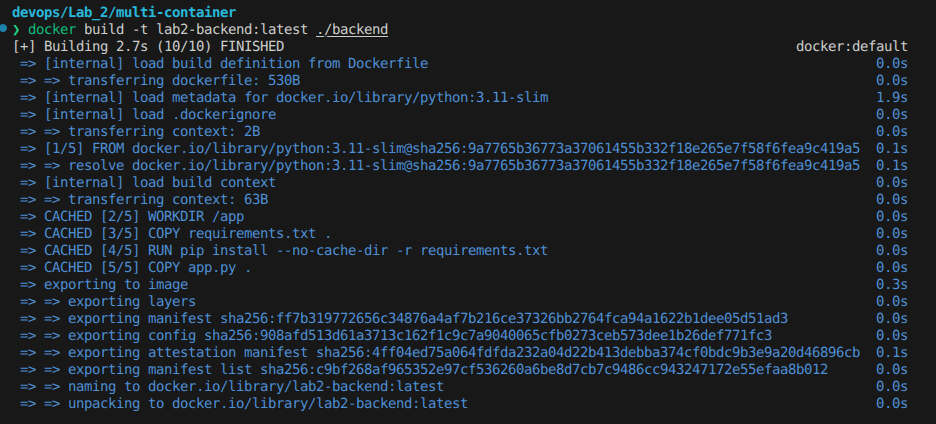
\includegraphics[width=0.85\textwidth]{images/docker_build_backend.png}
  \caption{Backend image built inside Minikube's Docker daemon}
  \label{fig:docker_build_backend}
\end{figure}

\begin{figure}[H]
  \centering
  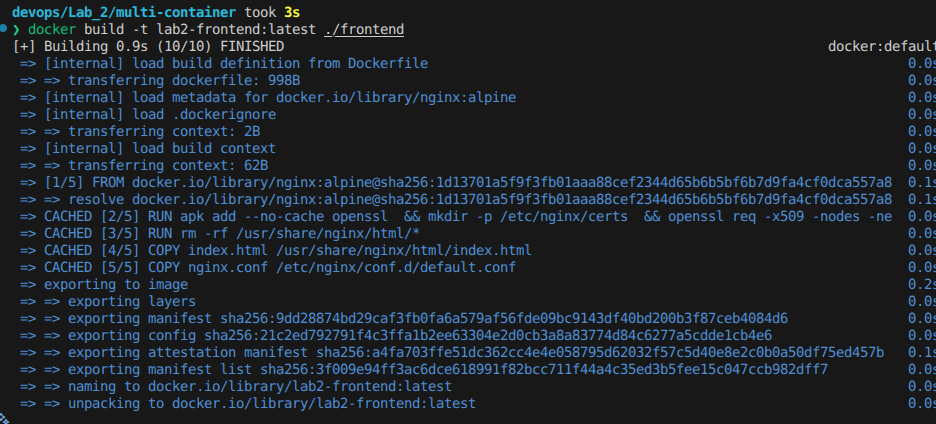
\includegraphics[width=0.85\textwidth]{images/docker_build_frontend.png}
  \caption{Frontend image built inside Minikube's Docker daemon}
  \label{fig:docker_build_frontend}
\end{figure}

% What to capture: build outputs showing the backend and frontend images were created successfully.

% ─────────────────────────────────────────────────────────────────────────────
\subsection{Kubernetes Manifest Files}
% ─────────────────────────────────────────────────────────────────────────────

All Kubernetes resources are defined as YAML manifests organised in a
\texttt{k8s/} directory and combined with a \texttt{kustomization.yaml} file:

\begin{verbatim}
k8s/
  namespace.yaml
  configmap.yaml
  secret.yaml
  database-init-configmap.yaml
  database-pvc.yaml
  database.yaml
  database-service.yaml
  backend.yaml
  backend-service.yaml
  frontend.yaml
  frontend-service.yaml
  kustomization.yaml
\end{verbatim}

% ── MySQL Secret ─────────────────────────────────────────────────────────────
\subsubsection{MySQL Secret}

Sensitive credentials are stored in a Kubernetes Secret rather than plain
environment variables:

\begin{lstlisting}[style=yamlstyle, caption={k8s/secret.yaml}]
apiVersion: v1
kind: Secret
metadata:
  name: db-credentials
  namespace: lab2
type: Opaque
stringData:
  MYSQL_ROOT_PASSWORD: "rootpassword"
  MYSQL_PASSWORD: "lab2pass"
  DB_USER: "lab2user"
  DB_PASSWORD: "lab2pass"
\end{lstlisting}

% ─────────────────────────────────────────────────────────────────────────────
\subsection{Building and Pushing Docker Images}
% ─────────────────────────────────────────────────────────────────────────────

The custom images from Lab~2 were rebuilt locally and loaded into Minikube so
that the Kubernetes cluster can use them without a remote container registry.

\begin{lstlisting}[style=bashstyle, caption={Build images inside Minikube's Docker context}]
# Point shell to Minikube's Docker daemon
eval $(minikube docker-env)

# Build backend image
docker build -t lab2-backend:latest ./backend

# Build frontend image
docker build -t lab2-frontend:latest ./frontend

# Load images into Minikube
minikube image load lab2-backend:latest
minikube image load lab2-frontend:latest

# Verify images are available locally
docker images | grep lab2
\end{lstlisting}

% ── SCREENSHOT: Docker build in Minikube ────────────────────────────────────
\begin{figure}[H]
  \centering
  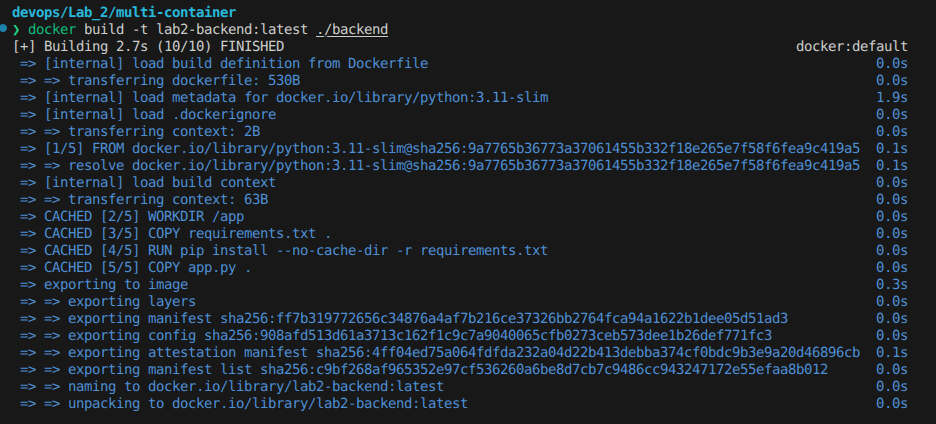
\includegraphics[width=0.85\textwidth]{images/docker_build_backend.png}
  \caption{Backend image built inside Minikube's Docker daemon}
  \label{fig:docker_build_backend}
\end{figure}

\begin{figure}[H]
  \centering
  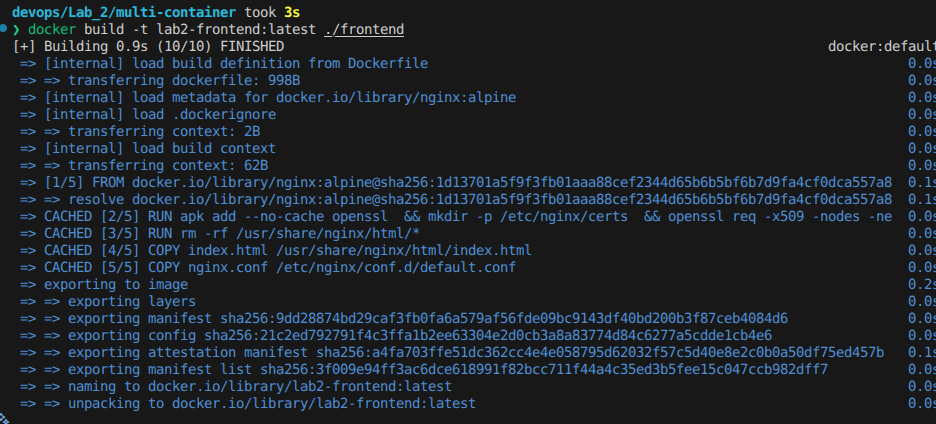
\includegraphics[width=0.85\textwidth]{images/docker_build_frontend.png}
  \caption{Frontend image built inside Minikube's Docker daemon}
  \label{fig:docker_build_frontend}
\end{figure}

% What to capture: build outputs showing the backend and frontend images were created successfully.

% ─────────────────────────────────────────────────────────────────────────────
\subsection{Kubernetes Manifest Files}
% ─────────────────────────────────────────────────────────────────────────────

All Kubernetes resources are defined as YAML manifests organised in a
\texttt{k8s/} directory and combined with a \texttt{kustomization.yaml} file:

\begin{verbatim}
k8s/
  namespace.yaml
  configmap.yaml
  secret.yaml
  database-init-configmap.yaml
  database-pvc.yaml
  database.yaml
  database-service.yaml
  backend.yaml
  backend-service.yaml
  frontend.yaml
  frontend-service.yaml
  kustomization.yaml
\end{verbatim}

% ── MySQL Secret ─────────────────────────────────────────────────────────────
\subsubsection{MySQL Secret}

Sensitive credentials are stored in a Kubernetes Secret rather than plain
environment variables:

\begin{lstlisting}[style=yamlstyle, caption={k8s/secret.yaml}]
apiVersion: v1
kind: Secret
metadata:
  name: db-credentials
  namespace: lab2
type: Opaque
stringData:
  MYSQL_ROOT_PASSWORD: "rootpassword"
  MYSQL_PASSWORD: "lab2pass"
  DB_USER: "lab2user"
  DB_PASSWORD: "lab2pass"
\end{lstlisting}

% ── Database StatefulSet and Service ────────────────────────────────────────
\subsubsection{Database StatefulSet and Service}

\begin{lstlisting}[style=yamlstyle, caption={k8s/database.yaml and k8s/database-service.yaml}]
apiVersion: apps/v1
kind: StatefulSet
metadata:
  name: mysql
  namespace: lab2
spec:
  serviceName: mysql
  replicas: 1
  selector:
    matchLabels:
      app: mysql
  template:
    metadata:
      labels:
        app: mysql
    spec:
      containers:
      - name: mysql
        image: mysql:8.0
        ports:
        - containerPort: 3306
          name: mysql
        env:
        - name: MYSQL_ROOT_PASSWORD
          valueFrom:
            secretKeyRef:
              name: db-credentials
              key: MYSQL_ROOT_PASSWORD
        - name: MYSQL_DATABASE
          valueFrom:
            configMapKeyRef:
              name: db-config
              key: MYSQL_DATABASE
        - name: MYSQL_USER
          valueFrom:
            configMapKeyRef:
              name: db-config
              key: MYSQL_USER
        - name: MYSQL_PASSWORD
          valueFrom:
            secretKeyRef:
              name: db-credentials
              key: MYSQL_PASSWORD
        volumeMounts:
        - name: mysql-data
          mountPath: /var/lib/mysql
        - name: init-script
          mountPath: /docker-entrypoint-initdb.d
        resources:
          requests:
            memory: "256Mi"
            cpu: "250m"
          limits:
            memory: "512Mi"
            cpu: "500m"
        livenessProbe:
          exec:
            command:
            - /bin/sh
            - -c
            - mysqladmin ping -h 127.0.0.1 -u root -p$MYSQL_ROOT_PASSWORD --protocol=TCP
          initialDelaySeconds: 60
          periodSeconds: 10
          timeoutSeconds: 5
          failureThreshold: 3
        readinessProbe:
          exec:
            command:
            - /bin/sh
            - -c
            - mysqladmin ping -h 127.0.0.1 -u root -p$MYSQL_ROOT_PASSWORD --protocol=TCP
          initialDelaySeconds: 40
          periodSeconds: 5
          timeoutSeconds: 5
          failureThreshold: 3
      volumes:
      - name: init-script
        configMap:
          name: db-init-script
  volumeClaimTemplates:
  - metadata:
      name: mysql-data
    spec:
      accessModes:
      - ReadWriteOnce
      resources:
        requests:
          storage: 5Gi
---
apiVersion: v1
kind: Service
metadata:
  name: mysql
  namespace: lab2
spec:
  clusterIP: None
  ports:
  - port: 3306
    targetPort: 3306
  selector:
    app: mysql
\end{lstlisting}

The database runs as a StatefulSet with a PVC, and the headless Service name
\texttt{mysql} is used for stable internal DNS resolution.

% ── Backend Deployment and Service ───────────────────────────────────────────
\subsubsection{Backend Deployment and Service}

\begin{lstlisting}[style=yamlstyle, caption={k8s/backend.yaml and k8s/backend-service.yaml}]
apiVersion: apps/v1
kind: Deployment
metadata:
  name: backend
  namespace: lab2
spec:
  replicas: 2
  selector:
    matchLabels:
      app: backend
  template:
    metadata:
      labels:
        app: backend
    spec:
      containers:
      - name: backend
        image: lab2-backend:latest
        imagePullPolicy: Never  # Use local image for development
        ports:
        - containerPort: 5000
        env:
        - name: DB_HOST
          valueFrom:
            configMapKeyRef:
              name: db-config
              key: DB_HOST
        - name: DB_PORT
          valueFrom:
            configMapKeyRef:
              name: db-config
              key: DB_PORT
        - name: DB_USER
          valueFrom:
            configMapKeyRef:
              name: db-config
              key: MYSQL_USER
        - name: DB_PASSWORD
          valueFrom:
            secretKeyRef:
              name: db-credentials
              key: DB_PASSWORD
        - name: DB_NAME
          valueFrom:
            configMapKeyRef:
              name: db-config
              key: DB_NAME
        resources:
          requests:
            memory: "128Mi"
            cpu: "100m"
          limits:
            memory: "256Mi"
            cpu: "200m"
        livenessProbe:
          httpGet:
            path: /api/health
            port: 5000
          initialDelaySeconds: 20
          periodSeconds: 10
          timeoutSeconds: 5
          failureThreshold: 3
        readinessProbe:
          httpGet:
            path: /api/health
            port: 5000
          initialDelaySeconds: 10
          periodSeconds: 5
          timeoutSeconds: 5
          failureThreshold: 3
---
apiVersion: v1
kind: Service
metadata:
  name: backend
  namespace: lab2
spec:
  type: ClusterIP
  ports:
  - port: 5000
    targetPort: 5000
    protocol: TCP
  selector:
    app: backend
\end{lstlisting}

The backend uses Flask and exposes a health endpoint at \texttt{/api/health}.

% ── Frontend Deployment and Service ──────────────────────────────────────────
\subsubsection{Frontend Deployment and Service}

\begin{lstlisting}[style=yamlstyle, caption={k8s/frontend.yaml and k8s/frontend-service.yaml}]
apiVersion: apps/v1
kind: Deployment
metadata:
  name: frontend
  namespace: lab2
spec:
  replicas: 2
  selector:
    matchLabels:
      app: frontend
  template:
    metadata:
      labels:
        app: frontend
    spec:
      containers:
      - name: frontend
        image: lab2-frontend:latest
        imagePullPolicy: Never  # Use local image for development
        ports:
        - containerPort: 80
        - containerPort: 443
        volumeMounts:
        - name: nginx-config
          mountPath: /etc/nginx/conf.d/default.conf
          subPath: default.conf
        resources:
          requests:
            memory: "64Mi"
            cpu: "50m"
          limits:
            memory: "128Mi"
            cpu: "100m"
        livenessProbe:
          httpGet:
            path: /
            port: 80
          initialDelaySeconds: 10
          periodSeconds: 10
          timeoutSeconds: 5
          failureThreshold: 3
        readinessProbe:
          httpGet:
            path: /
            port: 80
          initialDelaySeconds: 5
          periodSeconds: 5
          timeoutSeconds: 5
          failureThreshold: 3
      volumes:
      - name: nginx-config
        configMap:
          name: nginx-config
---
apiVersion: v1
kind: Service
metadata:
  name: frontend
  namespace: lab2
spec:
  type: ClusterIP
  ports:
  - name: http
    port: 8080
    targetPort: 80
    protocol: TCP
  - name: https
    port: 443
    targetPort: 443
    protocol: TCP
  selector:
    app: frontend
\end{lstlisting}

The frontend Service is exposed as a \texttt{ClusterIP} object and is accessed
locally using \texttt{kubectl port-forward} during testing.

% ─────────────────────────────────────────────────────────────────────────────
\subsection{Deploying All Resources}
% ─────────────────────────────────────────────────────────────────────────────

All manifests were applied to the cluster using the Kustomize overlay:

\begin{lstlisting}[style=bashstyle, caption={Applying all Kubernetes manifests}]
kubectl apply -k k8s/

# Verify all resources are created
kubectl get all -n lab2
kubectl get pods -n lab2
kubectl get svc -n lab2
\end{lstlisting}

% ── SCREENSHOT: kubectl apply output ───────────────────────────────────────
\begin{figure}[H]
  \centering
  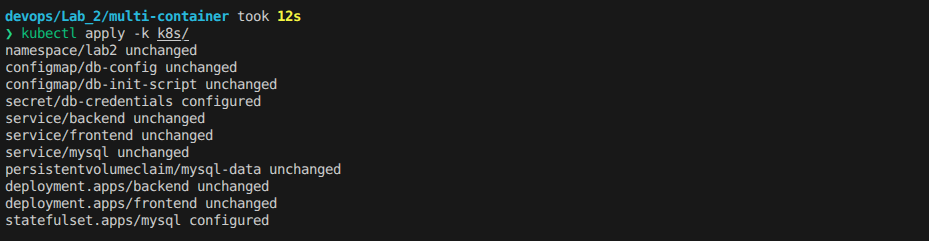
\includegraphics[width=0.85\textwidth]{images/run_all_kubectl.png}
  \caption{Output of \texttt{kubectl apply -k k8s/} showing resources created}
  \label{fig:kubectl_apply}
\end{figure}

\begin{figure}[H]
  \centering
  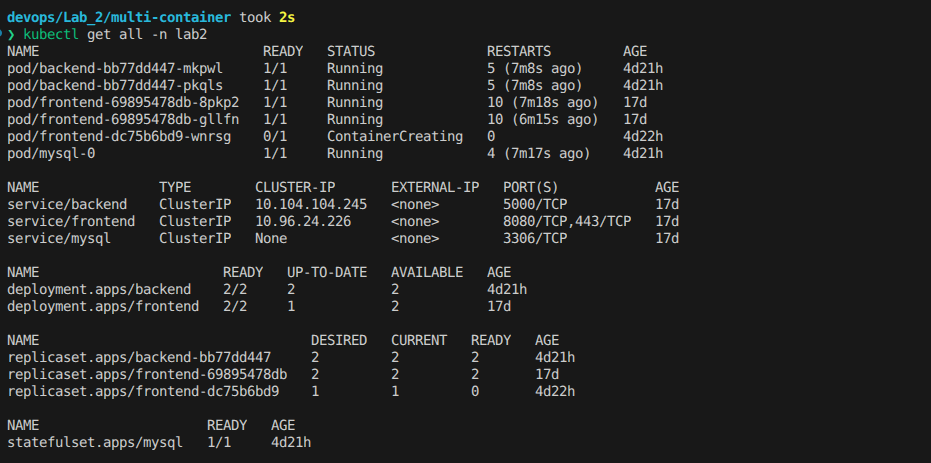
\includegraphics[width=0.85\textwidth]{images/kubectl_get_all.png}
  \caption{Output of \texttt{kubectl get all -n lab2} after deployment}
  \label{fig:kubectl_get_all}
\end{figure}
% What to capture: terminal showing resources created and then all pods/services/deployments in the namespace.

% ─────────────────────────────────────────────────────────────────────────────
\subsection{Verifying Pod and Service Status}
% ─────────────────────────────────────────────────────────────────────────────

\begin{lstlisting}[style=bashstyle, caption={Checking Pod and Service health}]
# Watch pods come up

# Describe a pod for detailed events
kubectl describe pod <pod-name>

# Check all services
kubectl get services
\end{lstlisting}

% ── SCREENSHOT: kubectl get pods ───────────────────────────────────────────
\begin{figure}[H]
  \centering
  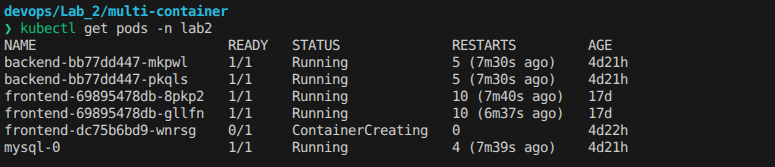
\includegraphics[width=0.85\textwidth]{images/kubectl_get_pods.png}
  \caption{All Pods in \texttt{Running} state with STATUS and READY columns}
  \label{fig:get_pods}
\end{figure}
% What to capture: `kubectl get pods` showing mysql, backend, and frontend
% pods all with STATUS=Running and READY=1/1.

% ── SCREENSHOT: kubectl get services ───────────────────────────────────────
\begin{figure}[H]
  \centering
  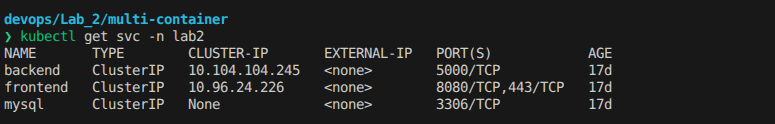
\includegraphics[width=0.85\textwidth]{images/kubectl_services.png}
  \caption{Services listing showing ClusterIP for db/backend and NodePort for frontend}
  \label{fig:get_services}
\end{figure}
% What to capture: `kubectl get services` showing db (ClusterIP), backend
kubectl apply -k k8s/

# Verify all resources are created
kubectl get all -n lab2
kubectl get pods -n lab2
kubectl get svc -n lab2

% =============================================================================
\section{Findings and Observations}
% =============================================================================

\begin{itemize}
  \item Kubernetes DNS automatically resolved the \texttt{db} hostname within
        the cluster, enabling the backend Pod to connect to MySQL without any
        IP address changes.

    \item Using \texttt{imagePullPolicy: Never} was essential to prevent Kubernetes
      from attempting to pull locally built images from a remote registry, which would
      result in \texttt{ErrImagePull} errors.

  \item The \texttt{depends\_on} directive from Docker Compose has no direct
        Kubernetes equivalent; an \textit{init container} or application-level
        retry logic is required to handle database readiness.

  \item Separating sensitive configuration into a \texttt{Secret} object is
        a significant security improvement over plain environment variables in
        Docker Compose files.

  \item Scaling the backend Deployment to three replicas demonstrated
        Kubernetes' load-balancing capability with no application downtime.
\end{itemize}

% =============================================================================
\section{Technical Challenges Encountered}
% =============================================================================

\begin{center}
\begin{tabular}{>{\bfseries}p{3.5cm} p{4.5cm} p{5cm}}
\toprule
Issue & Root Cause & Resolution \\
\midrule
\texttt{ErrImagePull} on backend Pod
  & Image not present in the local Minikube Docker context
  & Set \texttt{imagePullPolicy: Never} and rebuilt inside Minikube Docker context \\
\addlinespace
Backend \texttt{CrashLoopBackOff}
  & MySQL Pod not yet ready when backend started
  & Backend retries database connection during startup; verified with \texttt{kubectl logs} \\
\addlinespace
NodePort unreachable from host
  & Firewall blocking non-standard port
  & Used \texttt{minikube service frontend --url} to tunnel through Minikube \\
\addlinespace
\texttt{kubectl} version mismatch warning
  & Snap-installed kubectl version ahead of Minikube API server
  & Pinned kubectl version to match Minikube's Kubernetes version \\
\bottomrule
\end{tabular}
\end{center}

% =============================================================================
\section{Comparison: Docker Compose vs.\ Kubernetes}
% =============================================================================

\begin{center}
\begin{tabular}{>{\bfseries}p{3.5cm} p{4.5cm} p{4.5cm}}
\toprule
Feature & Docker Compose & Kubernetes \\
\midrule
Target environment & Single host, development & Multi-node, production \\
Configuration format & \texttt{docker-compose.yml} & Multiple YAML manifests \\
Service discovery & Service name (bridge network) & CoreDNS within cluster \\
Scaling & \texttt{--scale} flag & \texttt{kubectl scale} / HPA \\
Health management & Restart policies & Liveness / Readiness probes \\
Secret management & Environment variables & \texttt{Secret} objects \\
Load balancing & Basic round-robin & Service-level load balancing \\
\bottomrule
\end{tabular}
\end{center}

% =============================================================================
\section{Conclusion}
% =============================================================================

This lab successfully demonstrated the migration of a multi-container application
from Docker Compose to Kubernetes. Each service from Lab~2---frontend, backend,
and database---was re-deployed as a Kubernetes Deployment paired with an
appropriate Service type (ClusterIP or NodePort).

The exercise highlighted core Kubernetes concepts including declarative
configuration, built-in DNS-based service discovery, Secrets management, and
horizontal scaling. Although Kubernetes introduces greater operational complexity
than Docker Compose, it provides the robustness, scalability, and self-healing
capabilities required for production cloud-native workloads.

% =============================================================================
\end{document}
% =============================================================================